\documentclass{cdut_thesis}
\usepackage{listings} % 导入 listings 宏包,实现代码块
% 设置 listings 的全局样式
% 设置代码块样式
\lstset{
	language=TeX, % 语言设置为TeX
	basicstyle=\ttfamily, % 字体样式
	backgroundcolor=\color{gray!10}, % 背景色
	keywordstyle=\color{blue}, % 关键词颜色
	commentstyle=\color{green!60!black}, % 注释颜色
	showstringspaces=false, % 不显示字符串中的空格
	breaklines=true, % 自动断行
	numbers=left, % 行号位置
	numberstyle=\tiny\color{gray}, % 行号样式
	frame=single, % 代码块边框
	rulecolor=\color{black}, % 边框颜色
	xleftmargin=\parindent, % 左边距
}
\TitleCDUT{成都理工大学本科毕业论文非官方\LaTeX 模板}{Unofficial graduation thesis of Chengdu University of Technology \LaTeX template}
\KeywordCDUT{\LaTeX ;排版系统;毕业论文}{\LaTeX ;Typesetting system;Graduation thesis}% 注意用分号
\AuthorCDUT{姓名}
\StudentnumberCDUT{\quad}
\AdvisorCDUT{张三}{教授}
\MajorCDUT{数学与应用数学2班}
% 多少届的毕业生
\GradeCDUT{2024}

\begin{document}
%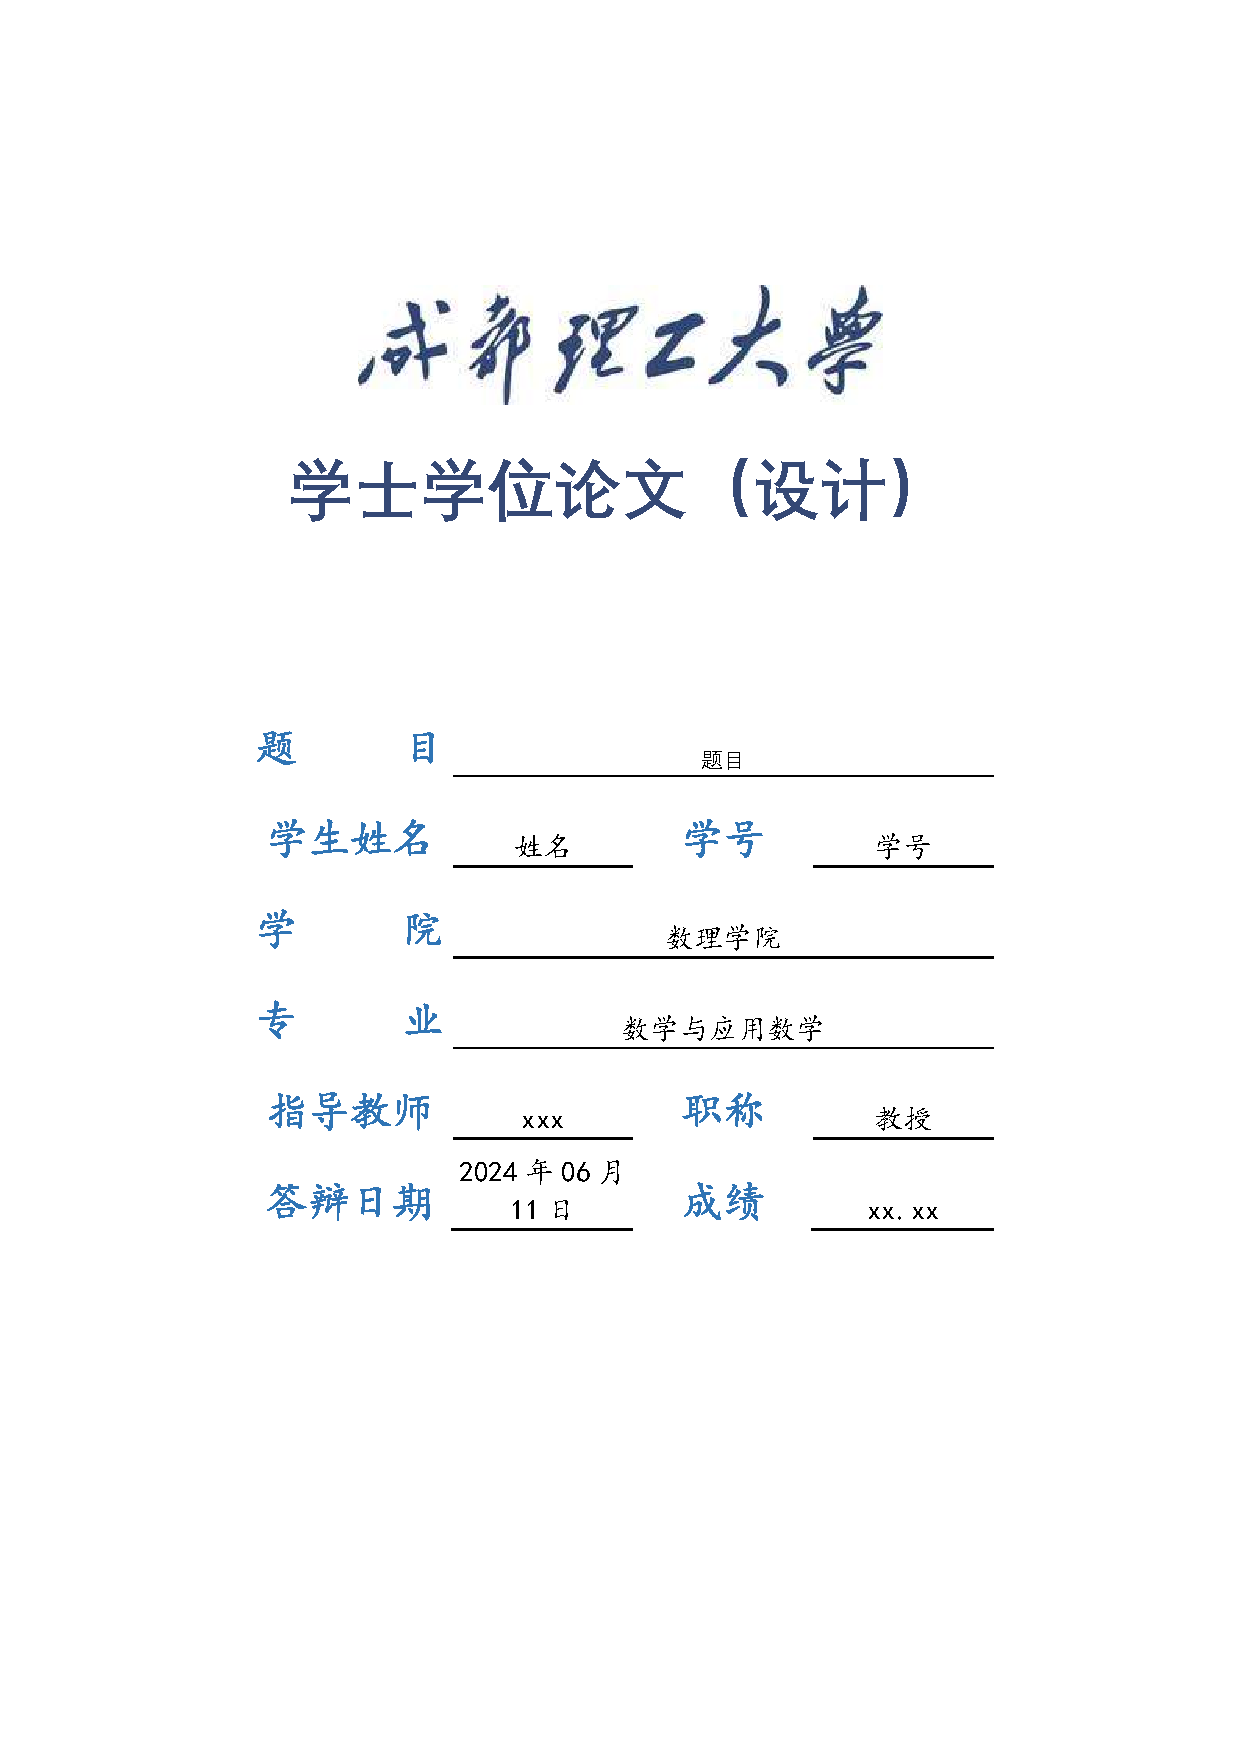
\includepdf{body/封面.pdf}% 不需要,若需要,将封面放到body中
% 摘要以及目录的页眉页脚
\fronthead
\makezhcover

\begin{chineseabstract}
%目的、方法、结果、意义
这是成都理工大学本科生毕业论文\textbf{非官方} \LaTeX 模板。
	
\textbf{v1.1:}本模板在\href{https://github.com/cs-whh/CDUT_thesis}{\color{red}GitHub:CDUT\_thesis项目}的基础上作了部分修改,以符合学校最新要求。
	
\textbf{注意:}本模板在编写过程中尽可能满足学校要求,由于原始规范主要针对Word。和\LaTeX 之间不可避免的差异加之编写者的水平有限,所以难免和学校提供的基于Word的样张存在细微差异,请谨慎使用!
\end{chineseabstract}



\begin{englishabstract}
This is an unofficial \ LaTeX template for graduate thesis of Chengdu University of Technology.
\end{englishabstract}


\newpage

\tableofcontents

\newpage
% 正文的页眉页脚
\texthead

%论文主体内容
\section{利用\LaTeX 排版中文文字}

\LaTeX 的源文件本质上是文本文档,利用Windows自带文本编辑器、note++、word、vim等文本编辑器均可编写出tex文档,至于texwork、texstudio、winedt等则为转述的tex编辑器,提供了语法高亮、匹配查找、自动补全命令等等用途。

除此之外\LaTeX 还可以排版数学公式、图片、表格等等,内容将在后续章节件数。
\subsection{\LaTeX 基本的命令与代码结构}
\LaTeX 命令均由反斜线$\backslash$开头,并为下列两种形式填空后续:
\begin{itemize}
	\item 由反斜线$\backslash$与一连串字母组成,如\verb|\LaTeX|。注意在命令后需加空格或其他非字母作分隔符;
	\item 由反斜线$\backslash$由后面的非字母符号组成,不需要分隔符,如\verb|\%|(百分号在\LaTeX 中为注释),为转义意。
\end{itemize}

注意\LaTeX 命令对\textbf{大小写是十分敏感的},比如输入\verb|\LaTeX|可以得到错落有致的\LaTeX 而输入\verb|\LaTex|或者\verb|\latex|则会报错,不会得到任何内容。

在\LaTeX 中的参数大多在$\{\cdots\}$或是在$[\cdots]$内,如之前所述\verb|\documentclass|\texttt{[CJK, GBK, UTF-8, oneside, a4paper, 12pt]{ctexart}}。
一些命令会在后面附带*号,带*号与不带*号结果不同。

为使一些状态、效果在局部生效,\LaTeX 引入了\textbf{环境}的用法,需要局部生效的内容被输入在环境内,由\verb|\begin{environment name}{arguments}|开始,由\verb|\end{environment}|结束。其中$environment$为环境名称,\verb|\begin{environment}|与\verb|\end{environment}|内的环境名应该一致,$arguments$为可选参数,环境之间允许嵌套使用。
\subsection{\LaTeX 排版中文}
排版中文文章时,与word不同,无需关注缩进、标题等等,在\LaTeX 中可以方便快捷的设置。一级标题设置代码为\verb|\section{title}|大括号内为一级标题的名称,对应的可以书写二级、三级标题,\LaTeX 命令分别为\verb|\subsection{title}|与\verb|\subsubsection{title}|。书写时,\LaTeX 会自动忽略文字中间的空格,在换行时需要多空一行。另外的,\LaTeX 中的注释为“\%”号。下面给出一个简短的例子。
\begin{verbatim}
\section{一级标题名称}
这里是第一章的内容
% 空一行代表分段,百分号在LaTeX中代表注释
这里是第一章的内容
\subsection{二级标题名称}
这里是1.1的内容
\end{verbatim}

用户可以将代码放置在本模板中进行尝试,需要注意的是,在body文件夹内新建文档并书写完后,需要在主文档中依照给定格式导入新书写的文档。

在\LaTeX 中书写中文,无需注意文章标题的编号,在\verb|\section{title}|类命令中,自带有计数器,可以为标题自动编号,这使得用户无需关注排版格式,更多的关注在文档内容上。
\subsection{常用环境}
\subsubsection{居中}
在\LaTeX 中有两种居中方式:
\begin{itemize}
	\item \verb|\centering|,在环境内使用,该环境内所有内容居中
	\item \verb|center| 环境,在环境内的所有内容居中
\end{itemize}
\begin{center}
	当使用了\verb|center|环境时候,环境内的所有内容都会被居中显示,且不会首行缩进。如果有特殊需要还可以使用flushleft 和flushright 环境,用于居左或者居右。
\end{center}
\subsubsection{带有编号的显示方式-列表(悬挂缩进)}
在书写论文时,经常会遇到需要分条叙述的方式,在一般书写排版中需要整体悬挂缩进。

在\LaTeX 中常用的两种环境,分别是itemize(无序)环境与enumerate环境(有序)两种环境可以互相嵌套使用,使用方法如下:
\begin{verbatim}
% itemize环境
\begin{itemize}
\item 第一条内容
\item 第二条内容
\end{itemize}
% enumerate环境
\begin{enumerate}[aa.]
\item 第一条内容
\item 第二条内容
\end{enumerate}
\end{verbatim}
itemize环境会给每一条内容前加$\bullet$,而enumerate环境可以自定义,如(1. 2. 3.或者是A. B. C.),对应的设置方法需要在环境后的参数中写\verb|1.|、\verb|A.|,需要注意的是在给enumerate环境添加参数时候需要导入enumerate包,否则只会有\verb|1. 2. 3.|的序号,并且无法设置样式。
\begin{itemize}
	\item 第一条内容
	\item 第二条内容
\end{itemize}
\begin{enumerate}[aa.]
	\item 第一条内容第一条内容第一条内容第一条内容第一条内容第一条内容第一条内容第一条内容第一条内容第一条内容第一条内容第一条内容第一条内容第一条内容第一条内容第一条内容
	\item 第二条内容
\end{enumerate}%第一章:绪论
\section{利用\LaTeX 排版图片与表格}
在介绍如何排版表格与图片时,先介绍浮动体的概念
\subsection{浮动体}
在排版中文文档或者实验报告时,尤其是在今后的论文、书籍撰写中,表格与图片均称为\textbf{浮动体}。顾名思义,浮动体在文中的位置不是固定的,美观起见需要自动放在合适的位置,在需要的时候做引用。在排版时,作者需要优先排版文字内容,最后再关注图片位置,不应固定死图片的位置,除了造成大片空白也会使得整体不够美观。
\subsubsection{浮动体的用法}
一般来说浮动体环境有两种,figure环境与table环境,分别用于浮动图片与表格,用法如下:
\begin{verbatim}
\begin{figure}[<placement>]
content...
\end{figure}
\end{verbatim}

表格与图片用法相同,跟在环境名后面的$placement$提供了浮动体在页面中允许排版的位置,默认为tbp,具体含义如表\ref{sec2:浮动体可选参数含义}。
\begin{table}[h!]
\caption{浮动体可选参数含义}
\label{sec2:浮动体可选参数含义}
\centering
\begin{tabular}{cc}
\hline
h&代码所处的当前位置\\
t&页面顶端\\
b&页码底部\\
p&单独成页\\
!&在决定位置时忽略限制\\
\hline
\end{tabular}
\end{table}
\subsubsection{浮动体的标题}
在浮动体中,利用\verb|\caption{...}|添加标题,用法与\verb|\section{...}|类似,添加的标题会自动编号,figure会在内容前显示如“图 1-1”的样式,表格类似。

紧跟着\verb|\caption{...}|后面可以添加\verb|\label{key}|命令交叉引用,具体在后面章节叙述。
\subsection{图片的排版}
\LaTeX 本身不支持插图功能,需要由graphicx 宏包(本模板已添加)辅助支持。在本模板下,可以添加.jpg.pdf.eps.png.bmp格式的图片,

在调用了graphicx包后,可以使用命令\verb|\includegraphics[⟨options⟩]{⟨filename⟩}|插入图片,$filename$是图片的位置,本模板中需要将图片放在figure文件中,并使用相对路径调用,如\verb|figure/filename.png|。$options$是需要的参数,如设置图片宽为0.7$cm$需要在该位置书写\verb|[width=0.7cm]|,具体的参数见表\ref{sec2:可选参数}。
\begin{table}[h]
\centering
\caption{可选参数}
\label{sec2:可选参数}
\begin{tabular}{lc}
\hline
参数&含义\\
\hline
width=h&将图片缩放到宽度为h\\
hight=h&将图片缩放到高度为h\\
scale=h&将图片按照原尺寸缩放h倍\\
angle=h&令图片逆时针旋转h度\\
\hline
\end{tabular}
\label{table1}
\end{table}

\begin{verbatim}
\begin{figure}[h]
\centering
\includegraphics[scale = 0.7]{example-image-A}
\caption{导入的图片}
\label{fig1}
\end{figure}
\end{verbatim}
\begin{figure}[h]
\centering
\includegraphics[scale = 0.7]{example-image-A}
\caption{导入的图片}
\label{fig1}
\end{figure}
需要排版并排子图推荐使用subfig宏包,具体使用请看宏包文档
\subsection{表格的排版}
在论文中,表格是比不可少的部分。下面给出一个简单的表格排版实例:
\begin{verbatim}
\begin{table}
\centering
\caption{表格排版实例}
\label{tab1}
\begin{tabular}{|c|l|r|}
\hline
AAA&B&CCC\\
\hline
A&BBB&C\\
\hline
\end{tabular}
\end{table}
\end{verbatim}

显示为表$^{[\ref{tab1}]}$。
\begin{table}[h]
\centering
\caption{表格排版实例}
\label{tab1}
\begin{tabular}{|c|l|r|}
\hline
AAA&B&CCC\\
\hline
A&BBB&C\\
\hline
\end{tabular}
\end{table}
与多行公式类似,表格排版中的列由tabular环境后的参数决定,c、l、r分别代表居中、居左、居右对齐,必须与列数相同,参数之间的竖线代表是否在表格中绘制竖线。行之间需要添加横线需要命令\verb|\hline|,如果需要合并单元格或者其他操作,具体见lshort表格排版章节,这里只讲述简单的部分。三线表的绘制只需要将参数中的竖线去除即可。

对于初次使用者而言,表格排版是一个很大的难题,在excel中有一个类似的插件可以快捷的生成大致的表格,在打开excel加载项后,下载插件\verb|excel2latex|即可。在生成大致表格后进行细微的调整,可以快速的绘制出想要的表格。%第二章:相关理论
\section{利用\LaTeX 排版数学公式}
在\LaTeX 中排版数学公式需要$amsmath$宏包(已经包含在本模板中),对多行公式的排版提供了有力的支持。在实验报告的书写中,主要以$amsmath$宏包的内容为主,其余内容不做阐述。
\subsection{公式排版基础}
在\LaTeX 中书写数学公式时必须带有数学环境,数学环境内可以识别特殊的命令并且字体改变为数学字体,一般数学环境有两种,书写方式如下:
\begin{itemize}
\item \textbf{行内公式:} 行内公式是出现在文字陈述中间的数学公式,需要用双\$符号括起来,例如我们知道对于矩阵而言,乘法交换率是不成立的,也就是说$\forall A\neq B,\, \exists A\times B\neq B\times A$(\verb|$A\times B\neq B\times A$|),书写时除去命令后必须的空格外,其他的空格会被一概忽略,至于如何添加空白会在后面叙述。
\item \textbf{行间公式:} 行间公式是出现在文字陈述段落中间的数学公式,一般需要编号。当行间公式需要编号时可以使用equation环境,不需要编号时可以使用简单的方式编写行间公式:\verb|\[myEquation\]|
\end{itemize}

在数学环境内,不允许有多于的空格与空行,需要强制空格可以使用命令\verb|\,|、\verb|\quad|、\verb|\qquad|等,他们的产生的空白距离有所不同。其次数学环境中的所有字母都会被当做变量处理,采用数学字体显示,当需要在数学环境中输入公式时,可以使用命令\verb|\text{}|。
\subsection{排版数学公式}
在以往的实验报告中,数学公式都会使用word中的mathtype书写,在较高的版本中可以复制mathtype为\LaTeX 代码,但这种投机取巧的方法写出来的符号会非常的丑,并且速度不会比直接使用\LaTeX 书写快多少。下面,作者会首先叙述一部分必要的知识,其次的内容会以实例的方式展现,需与tex文档(源文档)配合学习。

\begin{enumerate}[1.]
\item 上标的表示方式为\verb|a^{2}|,显示结果为$a^{2}$,当上标内容单一时可以省略大括号,如\verb|a^2|也可以显示为$a^2$,当需要输入符号$\^$时输入\verb|\^|即可。
\item 下表的表示方式为\verb|a_{2}|,显示结果为$a_{2}$,当小标内容单一时也可以省略大括号,当需要输入符号$\_$时输入\verb|\_|即可。
\item 同时需要上下标时书写没有先后顺序,\verb|a^{x+y}_{x_1}|与\verb|a_{x_1}^{x+y}|结果都是$a_{x_1}^{x+y}$。
\item 对于巨运算符,如果直接书写\verb|\sum^{n}_{i=1}n!|会容易显示为$\sum^{n}_{i=1}n!$,而添加命令\verb|\limits|后,\verb|\sum\limits^{n}_{i=1}n!|则会显示为$\sum\limits^{n}_{i=1}n!$。
\item 书写分数的命令为\verb|\frac{text}{den}|,其中text为分子部分,den部分为分母部分,如\verb|\frac{1}{2}|会显示为$\frac{1}{2}$,如果觉得分数略小可以适当的使用命令\verb|\dfrac{text}{den}|
显示为$\dfrac{1}{2}$。
\item 导数直接使用单引号即可\verb|f' f'' f'''|显示为$f' f'' f'''$,常见的运算符号与巨运算符如\verb|+ - \times \div = \sum \prod \int|,分别为$+ - \times \div = \sum \prod \int$,更多的基础符号见amsmath宏包或lshort,下面也给出了支持所有的符号大全与手写符号识别的网址。
\LaTeX 支持的符号大全:
\url{http://mirrors.ctan.org/info/symbols/comprehensive/symbols-a4.pdf}

手写符号识别:
\url{http://detexify.kirelabs.org/classify.html}
\item 需要输入大括号时需输入\verb|\{\}|。
\end{enumerate}
下面会用一些函数、习题、定理、证明过程或是计算过程作为实例:

\textbf{Stolz 定理}:设$\{y_n\}$是严格单调增加的正无穷大量,且
\[
\lim\limits_{n \to \infty}\frac{x_n-x_{n-1}}{y_n-y_{n-1}}=a\quad (a\text{可以为有限量,}+\infty\text{与}-\infty)\text{,}
\]
则
\[
\lim\limits_{n \to \infty}\frac{x_n}{y_n}=a\text{。}
\]

求极限
\[
\lim\limits_{n \to \infty}\frac{1^k+2^k+\cdots+n^k}{n^{k+1}}(k\text{为正整数})\text{。}
\]

由已知,可得
\begin{equation}\label{equ1}
\lim\limits_{n \to \infty}\frac{a^n}{n!}=0\text{。}
\end{equation}

设函数
\begin{equation}
	f(x)=\frac{x+e^{\frac{1}{x}}}{1+e^{\frac{4}{x}}}+\frac{\sin x}{|x|}
\end{equation}

问当$x\to 0$时,$f(x)$的极限是否存在?

设$f(x)$在$[a,b]$上连续,且$f(x)>0$,证明
\begin{equation}
\frac{1}{b-a}\int_{a}^{b}\ln f(x)\text{d}x\leqslant \ln \left(\frac{1}{b-a}\int_{a}^{b}f(x)\text{d}x\right)\text{。}
\end{equation}

常用的希腊字符如下:
\[\alpha \beta \gamma \delta \varepsilon \zeta \theta \eta \mu \xi \pi \sigma \omega \phi\]
\subsection{多行公式的排版}
在书写报告时,时长会遇到多行排版,如矩阵、分段函数等等,在下文将介绍部分常用的环境,用于排版多行公式。

多行排版的环境使用方式大致类似,需要对齐的位置利用$\&$分割,行末需要使用\verb|\\|分割。
\subsubsection{align环境}
align环境会给环境内的每一行公式编号,去掉编号可以使用\verb|\notag|,使用方式如下:
\begin{verbatim}{LaTeX}
\begin{align}
a & = b + c \\
a & = b + c \\
x + y & = d + e \notag
\end{align}
\end{verbatim}
显示为
\begin{align}
a & = b + c \\
a & = b + c \\
x + y & = d + e \notag
\end{align}

align环境会在$\&$符号处对齐,多个$\&$会分段对齐。
\subsubsection{aligned环境}
与align环境不同,aligned环境会给公式整体一个编号,而不是每一行都有编号,同时需要equation环境套在外面。
\begin{verbatim}
\begin{equation}
	\begin{aligned}
		a & = b + c \\
		x + y & = d + e 
	\end{aligned}
\end{equation}
\end{verbatim}
显示为
\begin{equation}
	\begin{aligned}
		a & = b + c \\
		x + y & = d + e 
	\end{aligned}
\end{equation}
split 环境和aligned 环境用法类似,也用于和equation 环境套用,区别是split 只能
将每行的一个公式分两栏,aligned 允许每行多个公式多栏。
\subsubsection{array环境}
array环境用于排版数学数组、矩阵等,数组可作为一个公式块,在外套用\verb|\left|、\verb|\right|等定界符。跟在环境名后的\verb|{cccc}|意为矩阵4列均居中(c代表居中、l代表左对齐、r代表右对齐,更仔细的将在表格排版处讲述),具体实例如下:
\begin{verbatim}
\[ 
\mathbf{X} = \left(
\begin{array}{cccc}
x_{11} & x_{12} & \ldots & x_{1n}\\
x_{21} & x_{22} & \ldots & x_{2n}\\
\vdots & \vdots & \ddots & \vdots\\
x_{n1} & x_{n2} & \ldots & x_{nn}\\
\end{array} \right) 
\]
\end{verbatim}
显示为
\[ 
\mathbf{X} = \left(
\begin{array}{cccc}
x_{11} & x_{12} & \ldots & x_{1n}\\
x_{21} & x_{22} & \ldots & x_{2n}\\
\vdots & \vdots & \ddots & \vdots\\
x_{n1} & x_{n2} & \ldots & x_{nn}\\
\end{array} \right) 
\]
其中,\verb|\left(|、\verb|\right)|就是矩阵的定界符,小括号可以替换为\verb|[ {|等。
\subsubsection{case环境}
借用之前所述的定界符,使用单侧定界符可以用来书写分段函数,如$\textbf{Riemann}$函数可以书写为:
\begin{verbatim}
\[
\mathbf{R}(x)=\left\{\begin{array}{ll}
\frac{1}{p},&x=\frac{q}{p}(p\in \mathbf{N}^{+},q\in \mathbf{Z}-\{0\},p,q\text{互质}),\\
1,&x=0,\\
0,&x\text{为无理数}
\end{array}\right.
\]
\end{verbatim}
显示为
\[
\mathbf{R}(x)=\left\{\begin{array}{ll}
\frac{1}{p},&x=\frac{q}{p}(p\in \mathbf{N}^{+},q\in \mathbf{Z}-\{0\},p,q\text{互质}),\\
1,&x=0,\\
0,&x\text{为无理数}
\end{array}\right.
\]
对于这类分段函数,可以使用更简单的cases环境来完成
\begin{verbatim}
\[
\mathbf{R}(x)=\begin{cases}
\frac{1}{p},&x=\frac{q}{p}(p\in \mathbf{N}^{+},q\in \mathbf{Z}-\{0\},p,q\text{互质}),\\
1,&x=0,\\
0,&x\text{为无理数}
\end{cases}
\]
\end{verbatim}
显示为
\[
\mathbf{R}(x)=\begin{cases}
\frac{1}{p},&x=\frac{q}{p}(p\in \mathbf{N}^{+},q\in \mathbf{Z}-\{0\},p,q\text{互质}),\\
1,&x=0,\\
0,&x\text{为无理数}
\end{cases}
\]%第三章:应用实践
\section{v1.1的重要修改内容:文献引用}
\textbf{2024年06月20日}:原版本的引用格式采用的是\textcolor{red}{顺序-编码制},与学校要求不符。本模板将引用格式修改为\textcolor{red}{著者-出版年制}。使用前置条件如下:
\subsection{制作或者生成bib文件}

\subsubsection{手动制作}
例如:
\begin{lstlisting}
@article{wanger2009,
	author    = {王二 and 张三 and 李四},
	key       = {wang2 er4 and zhang1 san1 & li3 si4},
	title     = {单引用测试,标题1},
	journal   = {journal},
	year      = {2010}	
	}
\end{lstlisting}
\begin{itemize}
	\item wanger2009:是文章的标签,引用时通过它,可以对应到文章。
	\item author:作者名称,不同作者按顺序用and分隔开。
	\item key:作者的拼音,数字表示声调。方便按拼音顺序排列参考文献
	\item title:文章标题
	\item journal:期刊名称
	\item year:出版年份
	...
\end{itemize}
不建议使用这种方式,挺麻烦的
\subsubsection{自动制作}
在阅读文献时使用zotero、endnote等文献管理器对文献进行管理,后期可以选中需要的文件一键导出参考文献的bib文件(如图\ref{参考文献导出示意图})。

\begin{figure}[h]
	\centering
	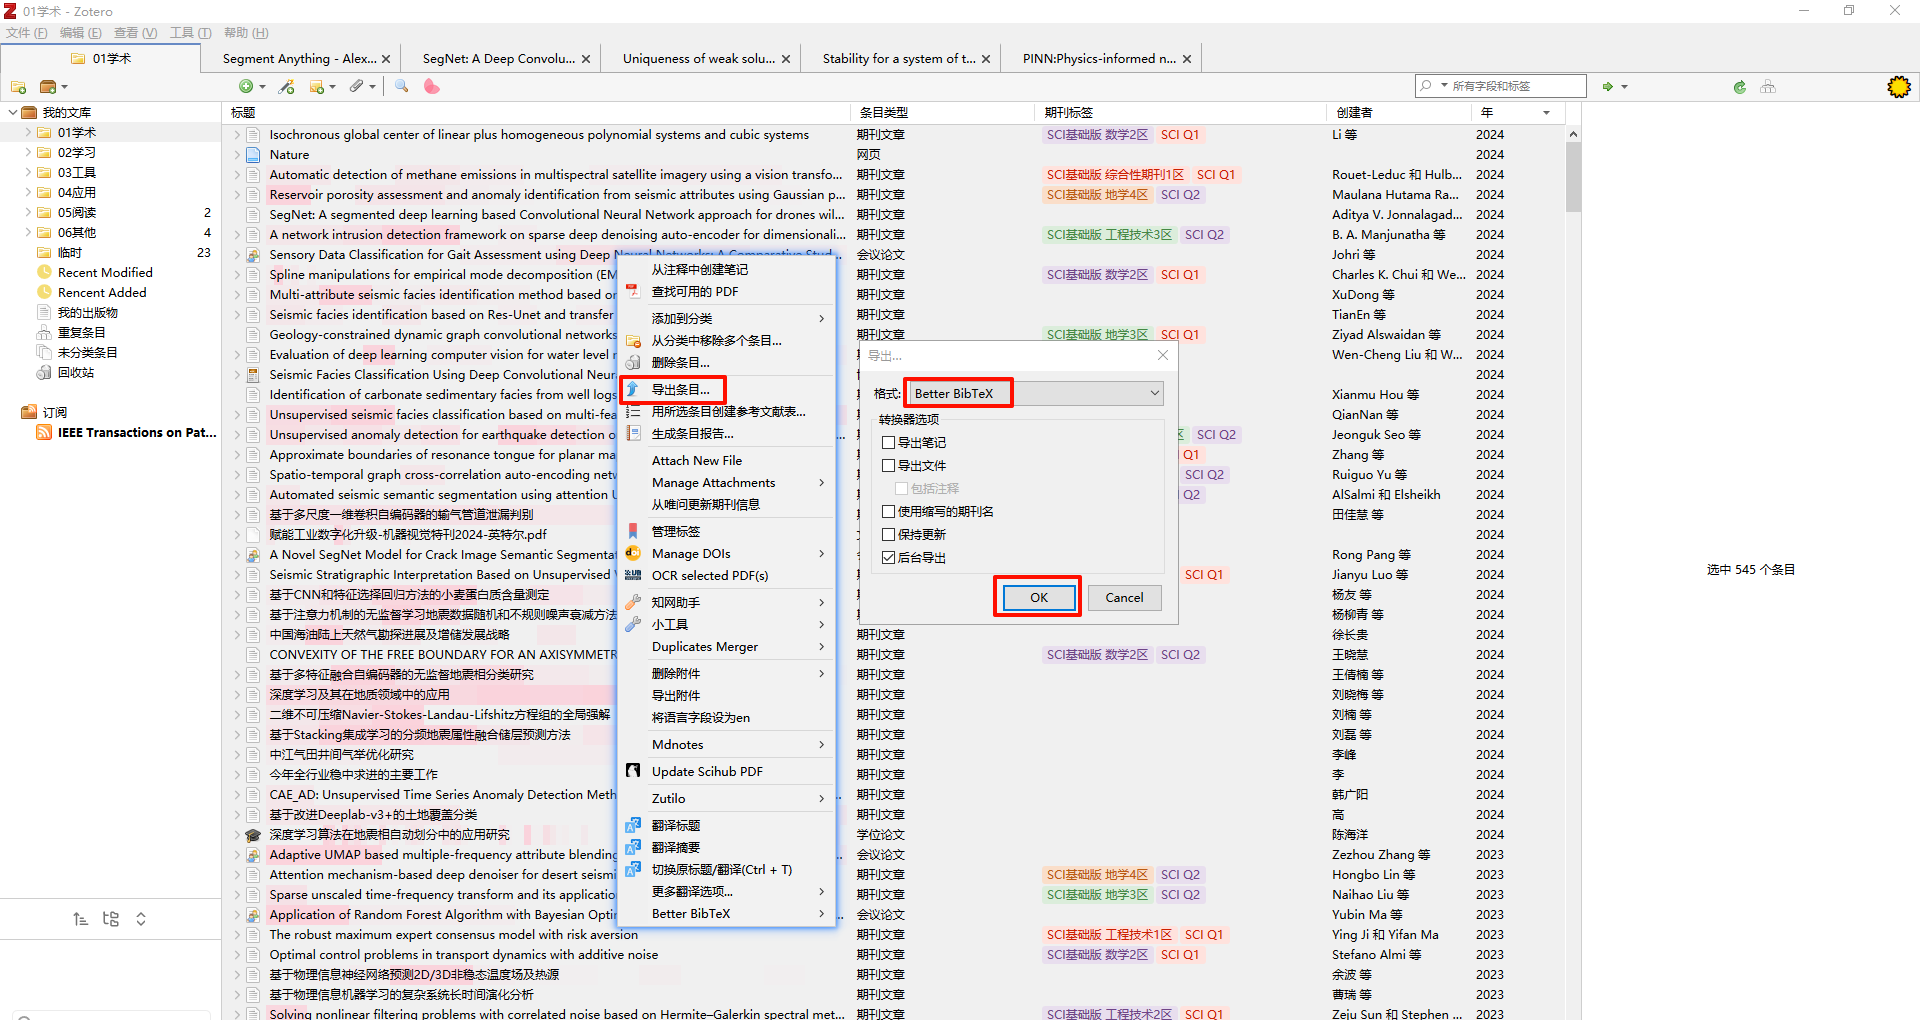
\includegraphics[width = 14cm]{figures/参考文献.png}
	\caption{zotero一键导出参考文献的bib文件}
	\label{参考文献导出示意图}
\end{figure}

\subsubsection{注意}
单独强调一下:无论是手动制作还是自动生成bib文件,只要是中文文献,就要手动加\textbf{key}值,以保证\textbf{中文文献在参考文献目录中能够按照拼音顺序排列}。例如:
\begin{lstlisting}
	@article{wanger2009,
		author    = {王二 and 张三 and 李四},
		key       = {wang2 er4 and zhang1 san1 & li3 si4},
	}
\end{lstlisting}
\subsection{两种引用格式}
有了bib文件,就可以在论文中插入引用了。假设最终需要引用的文献的bib文件如下:
\begin{lstlisting}
@article{wanger2009,
	author    = {王二 and 张三 and 李四},
	key       = {wang2 er4 and zhang1 san1 & li3 si4},
	title     = {单引用测试,标题1},
	journal   = {journal},
	year      = {2010}	
}
@article{zhangsan2010,
	author    = {张三 and 李四},
	key       = {zhang1 san1 & li3 si4},
	title     = {多引用测试,标题1},
	journal   = {journal},
	year      = {2010}	
}
@article{lisi2011,
	author    = {李四 and 张三},
	key       = {li3 si4 & zhang1 san1},
	title     = {多引用测试,标题2},
	journal   = {journal},
	year      = {2011}	
}
\end{lstlisting}
\subsubsection{第一种引用形式}
\textbf{示例1:}\cite{wanger2009}这是第一种引用形式。
\begin{lstlisting}
\cite{wanger2009}
\end{lstlisting}

\subsubsection{第二种引用形式}
\textbf{示例2:}这是第二种引用形式\citep{wanger2009}。
\begin{lstlisting}
\citep{wanger2009}
\end{lstlisting}

\textbf{示例3:}这是第二种引用形式\citep{wanger2009,zhangsan2010,lisi2011},引用多篇佐证本文观点。
\begin{lstlisting}
\citep{wanger2009,zhangsan2010,lisi2011}
\end{lstlisting}

写作时基本是用这两种引用形式,,英文文献与上面引用一致(会自动处理成英文版本)。

\textbf{示例4:}英文文献示例\citep{LiK2019}。
\begin{lstlisting}
\citep{LiK2019}
\end{lstlisting}


注意:只要bib文件是严格按照要求制作的,就不会在这里出现错误。所以最好学习使用文献管理器制作bib文件,而非手动制作。
\subsection{参考文献目录}

只要bib文件是严格正确的,参考文献目录会自动生成符合规定(中文在上,外文在下。文献名称按顺序排列下来等规则)的参考文献目录。所以这里不需要过多关注。

bib文件放在body文件夹中,其名称为:refer.bib。
\begin{lstlisting}
\phantomsection
\bibliography{body/refer.bib}
\end{lstlisting}

\section{v1.1的其他修改内容:一些格式上的调整}
\begin{itemize}
	\item 图、表、公式的caption采用"-"作为分隔符,比如:图1-1,表2-2,公式3-3,符合学校规定。
	\item 修改页眉内容:“成都理工大学20xx届学士学位论文(设计)”,符合学校规定
	\item 目录跳转问题:原模板在结论、致谢、参考文献等无法实现点击跳转,本模板解决了这个问题。
	\item 目录的其他问题:原模板引导点("......")过长,本模板作了调整,适合论文页码的位数$\le2$的论文;原模板目录会添加“摘要”、“目录”进目录,实际不需要。本模板作了删除处理。
	\item 页面距离的问题:原模版的文字到页眉距离过大,本模板将这段距离适当调小,看起来更为美观。由于页眉、页脚距离与word的原理不一样,所以这里面还存在着问题,需要后续进一步修改,以使得latex的排版结果与word一致。(其实影响不大,能解决最好)
	
\end{itemize}
%结论、致谢、参考文献
\begin{conclusion}
这里写结论。
\end{conclusion}
\begin{thanks}
感谢老师感谢老师感谢老师感谢老师感谢老师感谢老师感谢老师感谢老师感谢老师。
\end{thanks}

% 引用 .bib 文件


\phantomsection
\bibliography{body/refer.bib}
%\appendix
\section{代码}

\subsection{附录二级标题}
附录内容附录内容附录内容附录内容附录内容附录内容

\section{数据}
附录内容附录内容附录内容附录内容附录内容附录内容附录内容附录内容附录内容附录内容附录内容附录内容%附录。一般可以没有
\end{document}

